\documentclass[a4paper,12pt]{article}
\usepackage[left=4cm,right=2cm,top=2cm,bottom=2cm,includefoot]{geometry}	%Seitenränder
\usepackage[ngerman]{babel}													%deutschsprachig + Umlaute
\usepackage{amsmath}														%mathematische Formeln
\usepackage{graphicx} 														%einfügen von Bildern und Grafiken
\usepackage{subfig}														%einfügen von Bildern und Grafiken nebeneinander
\usepackage[onehalfspacing]{setspace}										%Zeilenabstand 1,5
%\usepackage[authoryear]{natbib} 											%Literaturreferenzen
\usepackage[subfigure]{tocloft}												%Manupulation Inhaltsverzeichnis
\usepackage{eurosym}														%Darstellung Eurosymbol
\usepackage{caption} 														%Manupulation von Benennungen/captions
\usepackage{pdfpages}														%Einbinung von PDF-Dokumenten
%\usepackage{tikz}															%Erstellung und Darstellung von Diagrammen
%\usepackage{pgfplots}  														%Plotten von Graphen
%\pgfplotsset{compat=1.16}													%Zusatzpacket von pgfplots
\usepackage{pdflscape}														%Darstellung von Seiten im Querformat
\usepackage{tabularx}
\usepackage{color}															%Textfarbe ändern
\usepackage[colorlinks=true,linkcolor=blue]{hyperref}						%Links und Querverweise im Dokument

\setlength\parindent{0pt}													%kein Einrücken bei Absatzanfang

\begin{document}
\begin{titlepage}															%Beginn der Titelseite
	%\begin{figure}[h]
		%\includegraphics[width=1\textwidth]{Bild.jpg}						%Einfügen eines Titelbildes
	%\end{figure}

\vfill

\begin{center}
	{\textbf{\LARGE{Dokumentation I\&K Projekt\\ {\flqq Learning Spaces\frqq}}}}
\end{center}

\vfill
\textbf{Hochschule für Technik und Wirtschaft des Saarlandes}\\
\textbf{Fakultät für Wirtschaftswissenschaften}\\
\textbf{Studiengang: Wirtschaftsingenieurwesen}\\
\vfill

\begin{tabular}{lc}
Name & 123456 \\
Name & 123456 \\
Name & 123456 \\
Name & 123456 \\
Name & 123456 \\
\end{tabular}\\

\end{titlepage}																%Ende der Titelseite

\thispagestyle{empty}
\newpage 																	% Seitenumbruch

\renewcommand{\thesection}{\Roman{section}}
\pagenumbering{gobble}

%\addcontentsline{toc}{section}{Inhaltsverzeichnis}
%\addcontentsline{toc}{section}{Abbildungsverzeichnis}
%\addcontentsline{toc}{section}{Tabellenverzeichnis}
%\addcontentsline{toc}{section}{IV Abkürzungsverzeichnis}
%\newpage

\tableofcontents
\pagestyle{plain}
\clearpage
%\listoffigures
%\clearpage
%\listoftables
%\clearpage

\setcounter{section}{0}
\renewcommand{\thesection}{\arabic{section}}
\pagenumbering{arabic}

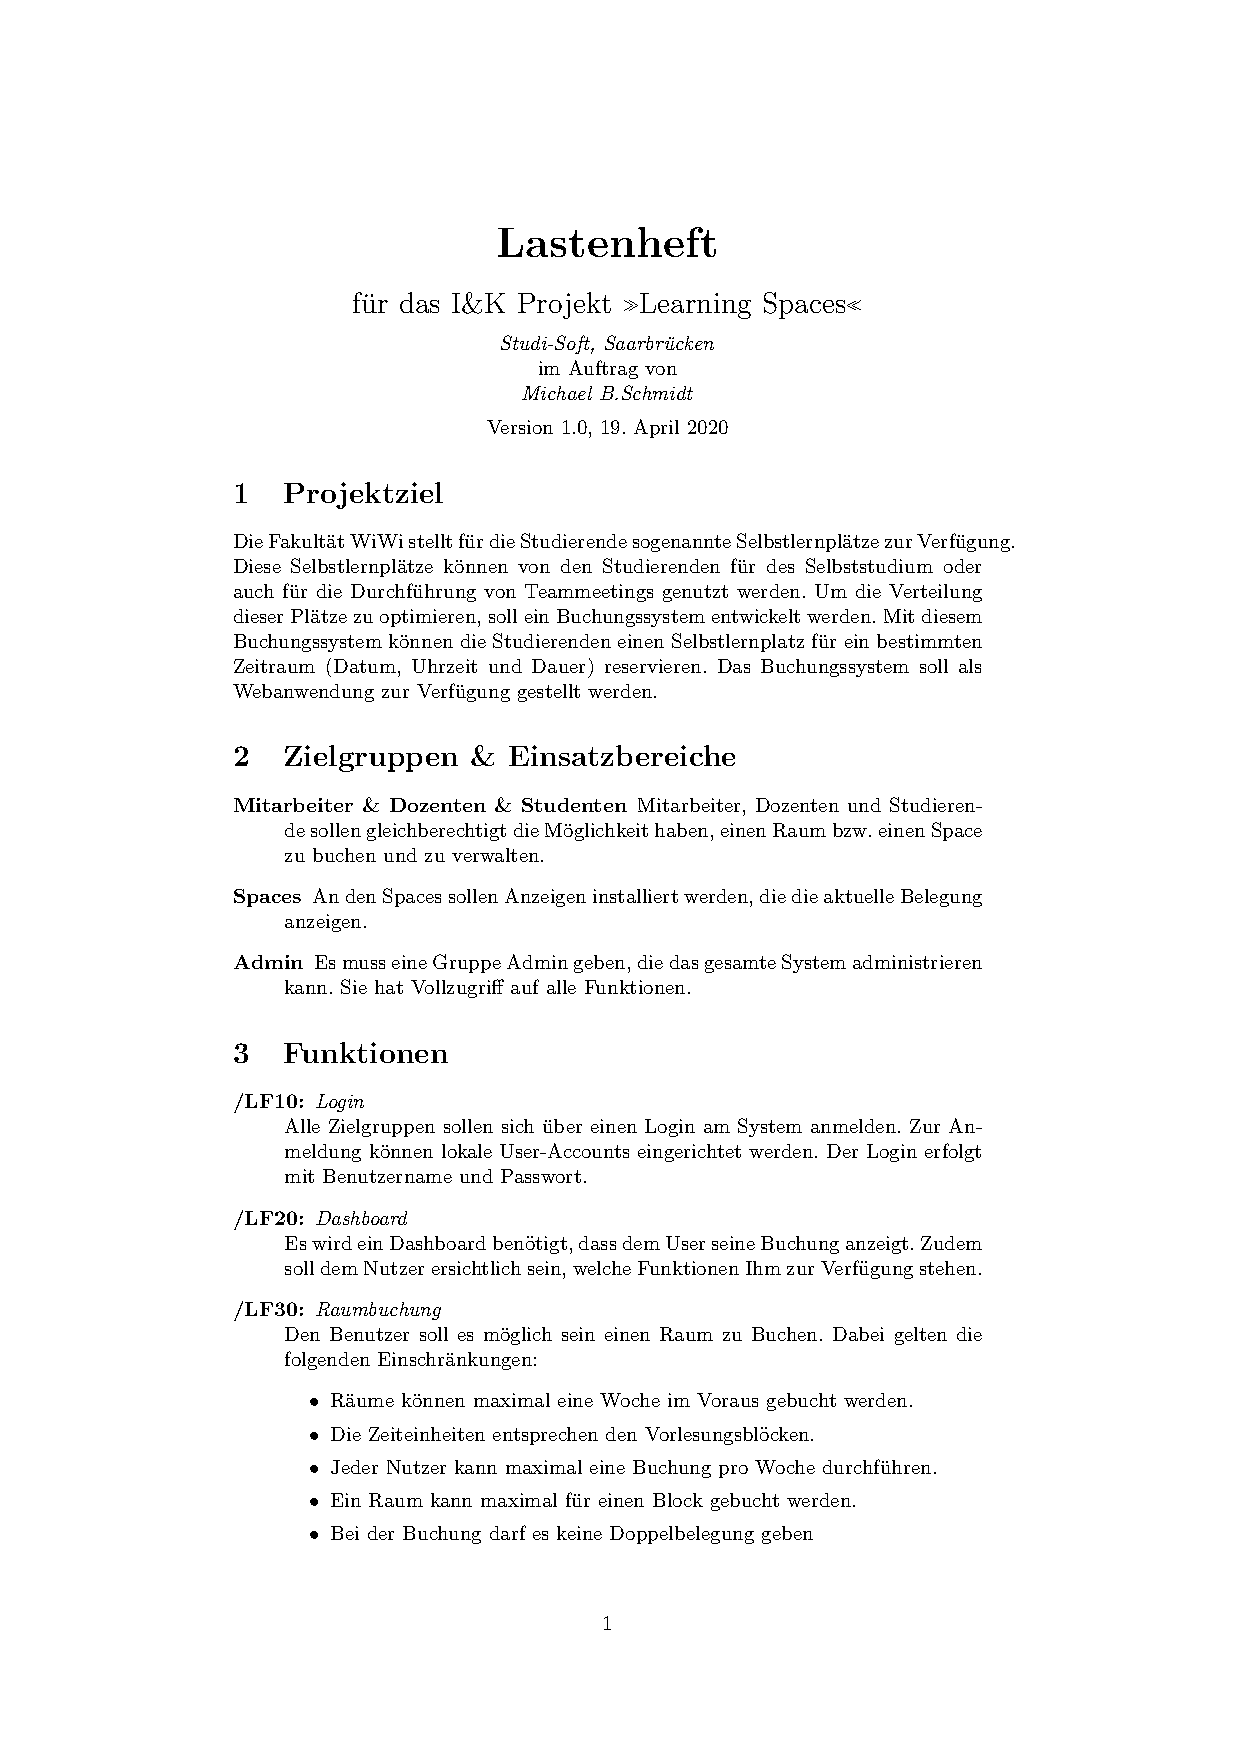
\includepdf[pages=1,scale=1,pagecommand={\section{Lastenheft}}]{PDF/Lastenheft_IuK}
\includepdf[pages=2,scale=1,pagecommand={\thispagestyle{plain}}]{PDF/Lastenheft_IuK}

\section{Pflichtenheft}

\section{Kapitel 3}
\end{document}